\documentclass[11pt,a4paper]{article}

% ---------------------------------------------------------------- packages
\usepackage[T1]{fontenc}
\usepackage[utf8]{inputenc}
\usepackage{newtxtext,newtxmath}
\usepackage[scaled=0.86]{inconsolata}
\usepackage[a4paper,margin=2.35cm,top=2.2cm,bottom=2.4cm]{geometry}
\usepackage{microtype}
\usepackage{amsmath}
\usepackage{booktabs,array,multirow,tabularx}
\usepackage{graphicx}
\usepackage[table]{xcolor}
\usepackage{tikz}
\usetikzlibrary{arrows.meta,positioning,calc,fit,backgrounds,shapes.geometric}
\usepackage[font=small,labelfont=bf,labelsep=period,skip=5pt]{caption}
\usepackage{subcaption}
\usepackage{enumitem}
\usepackage[compact]{titlesec}
\usepackage{fancyhdr}
\usepackage[hidelinks]{hyperref}
\usepackage[capitalise,noabbrev]{cleveref}

% ---------------------------------------------------------------- style
\definecolor{accent}{HTML}{1F4E79}
\definecolor{ringc}{HTML}{6C8EBF}
\definecolor{cannonc}{HTML}{3C8D5A}
\definecolor{tdc}{HTML}{D08C2C}
\definecolor{directc}{HTML}{B5367A}
\definecolor{rowgray}{HTML}{F3F5F8}
\hypersetup{colorlinks=true,linkcolor=accent,citecolor=accent,urlcolor=accent}

\titleformat{\section}{\large\bfseries\color{accent}}{\thesection}{0.7em}{}
\titleformat{\subsection}{\normalsize\bfseries}{\thesubsection}{0.6em}{}
\titleformat{\paragraph}[runin]{\normalsize\bfseries}{}{}{}[.]
\titlespacing*{\section}{0pt}{1.3ex plus .4ex}{0.7ex}
\titlespacing*{\subsection}{0pt}{1.0ex plus .3ex}{0.4ex}
\titlespacing*{\paragraph}{0pt}{0.6ex}{0.6em}

\setlist{nosep,leftmargin=1.3em,topsep=2pt}
\setlength{\parskip}{0pt}
\renewcommand{\arraystretch}{1.12}
\setlength{\tabcolsep}{5pt}

\pagestyle{fancy}
\fancyhf{}
\fancyhead[L]{\small\color{gray}CEG5206 Team Project, Group 7}
\fancyhead[R]{\small\color{gray}Data Layout and Communication Cost of Distributed Matrix Multiplication}
\fancyfoot[C]{\small\thepage}
\renewcommand{\headrulewidth}{0.3pt}

\newcommand{\todo}[1]{\textcolor{red}{[#1]}}
\newcommand{\code}[1]{\texttt{#1}}
\newcommand{\Ccrit}{C_{\mathrm{crit}}}
\newcommand{\Ctot}{C_{\mathrm{total}}}
\newcommand{\Wcrit}{W_{\mathrm{crit}}}
\newcommand{\Ftot}{F_{\mathrm{total}}}
\newcommand{\repo}{\url{https://github.com/ceg5206-g7/dmm}}

\begin{document}

% ================================================================ title
\thispagestyle{plain}
\begin{center}
  {\small\color{gray}CEG5206 Algorithms \& Performance Optimization for Computing \textperiodcentered{} AY2026/27 Semester 1}\\[0.9ex]
  {\LARGE\bfseries\color{accent} Data Layout and Communication Cost of\\[0.3ex] Distributed Matrix Multiplication}\\[1.4ex]
  {\large Group 7: Yang Tingjie \quad Yang Hanwei \quad Meng Xiangrun \quad Jin Ceyang}
\end{center}

\vspace{0.4ex}
\noindent
\begin{tabularx}{\textwidth}{@{}>{\bfseries\small}l>{\small\raggedright\arraybackslash}X@{}}
\toprule
Repository      & \repo \quad(source, tests, build/run instructions, configuration files) \\
Submitted version & commit \href{https://github.com/ceg5206-g7/dmm/commit/0b8b2b8df622842b03d3e398593a7c3504770e75}{\code{0b8b2b8}}, release \href{https://github.com/ceg5206-g7/dmm/releases/tag/experiment-results-0b8b2b8}{\code{experiment-results-0b8b2b8}}; later commits on \code{main} add only result data and this report \\
Experiment data & x86 run: \code{dmm\_local\_lowload\_results\_2026-11-10/} on \code{main}; ARM64 run: release \href{https://github.com/ceg5206-g7/dmm/releases/tag/experiment-results-9fc781b}{\code{experiment-results-9fc781b}}; CSV copies and figure script: \code{report/} \\
Documentation   & \url{https://ceg5206-g7.github.io/dmm_doc/} \\
\bottomrule
\end{tabularx}

\vspace{1.2ex}
\begin{abstract}
\noindent
Distributing a dense matrix product over $P$ processors leaves the arithmetic unchanged, but the data
layout determines how much each node communicates, how often the nodes synchronise and how much memory
each node needs. We implement the 1D ring, Cannon's 2D algorithm and the replicated 2.5D algorithm on one
bulk-synchronous-parallel (BSP) runtime in C++20, together with 2.5D-direct, a variant of our own that
replicates and reduces through all nodes instead of through a base layer. Every run multiplies real FP32
data and copies real messages, and the recorded trace allows one execution to be priced for any machine
parameters. All 39 formal configurations agree with an FP64 reference. Under a tight budget of $8n^2/P$
words per node, Cannon is the cheapest layout in every scenario. With $32n^2/P$ words, the textbook 2.5D
route still wins only 3 of the 72 parameter combinations, because its base-layer collectives lie on the
critical path; 2.5D-direct removes them, lowers the critical communication at $P=256$ from 64 to 28 units
of $n^2/P$, 20\% below Cannon, and wins 28 of the 72 combinations. Measurements with four workers on an x86 and an ARM64 host reach a $3.5$--$4.0\times$
speedup at $n=1024$ and show that, on shared-memory hosts, barriers rather than data movement limit small
problems.
\end{abstract}

% ================================================================ 1
\section{Introduction}
\label{sec:intro}

Dense matrix multiplication is the core of every linear layer in a neural network, and its distributed
form underlies tensor parallelism. Once the operands are divided among $P$ processors the arithmetic is
fixed at $2n^3$ FLOPs; the data layout decides how many words each node must receive, how many
synchronisation rounds are needed and how much data each node holds at once. These costs pull in
different directions. A 1D row layout needs no rearrangement but moves $\Theta(n^2)$ words through every
node. Two-dimensional layouts such as Cannon's algorithm~\cite{cannon1969,vandegeijn1997} reduce this to
$\Theta(n^2/\sqrt P)$, and the 2.5D algorithm of Solomonik and Demmel~\cite{solomonik2011} saves a further
factor $\sqrt c$ by replicating the inputs $c$ times, at the price of $c$ times more memory and an
additional reduction~\cite{ballard2011,ballard2014}.

Asymptotic statements of this kind do not tell a practitioner which layout to choose for a given problem
and machine. Our research question is therefore practical: \emph{for a given matrix size, number of
nodes and per-node memory budget, does the communication saved by replication outweigh the cost of
replication, reduction and layout conversion, and how does the answer change as communication and
synchronisation become more expensive?} We answer it by executing all layouts on one runtime and pricing
their exact executed costs, rather than by comparing separate programs or textbook formulas.

\paragraph{Contributions}
\begin{itemize}
\item A BSP plan runtime in which each layout is a single schedule-building function. All layouts share
      the GEMM kernel, message handling, memory ledger and timing boundary, so measured differences come
      from the layout alone (\cref{sec:impl}).
\item Executed and validated counts of work, communication, supersteps and live memory for four layouts,
      checked against closed-form expressions and an independent FP64 oracle (\cref{sec:impl,sec:verify}).
\item 2.5D-direct, a replication schedule that removes the base-layer bottleneck of the textbook 2.5D
      route and makes replication the cheapest choice in 28 parameter combinations instead of 3
      (\cref{sec:direct}).
\item A budget-filtered layout selection over 144 combinations of matrix size, grid, cost parameters and
      memory budget, and calibrated wall-clock measurements on an x86 and an ARM64 host, with an analysis
      of when replication pays and where the BSP model falls short (\cref{sec:results,sec:discussion}).
\end{itemize}

% ================================================================ 2
\section{Problem and Cost Model}
\label{sec:model}

We compute $C=AB$ for dense $n\times n$ FP32 matrices and count a multiply--add as two FLOPs. $P$ logical
nodes, numbered in row-major order, own private storage, and data crosses node boundaries only through
explicit message copies. All layouts start from and return to the same \emph{common distribution}, in
which node $r$ owns rows $[rN/P,(r+1)N/P)$ of $A$, $B$ and $C$; a layout that works on tiles must pay for
the conversion inside the measured route. Sizes that are not multiples of $P$ are zero-padded to
$N=\lceil n/P\rceil P$ and the result is cropped. The number of logical nodes $P$ is independent of the
number of worker threads $H$. When $P>H$ the nodes are executed in batches, which is valid for
correctness and counting but not for timing.

\paragraph{BSP cost}
A computation proceeds in supersteps of local work, message exchange and a barrier~\cite{valiant1990,hill1998}.
Let $F(r,s)$ be the FLOPs of node $r$ in superstep $s$ and $h(r,s)$ the larger of the words it sends and
receives. The modelled time is
\begin{equation}
T_{\mathrm{BSP}} = \sum_s\Big[w\max_r F(r,s) + g\max_r h(r,s) + l\Big] = w\,\Wcrit + g\,\Ccrit + l\,S,
\label{eq:bsp}
\end{equation}
where $w$, $g$ and $l$ are the costs of one FLOP, one word and one barrier. We report the normalised cost
$T_{\mathrm{BSP}}/w=\Wcrit+\gamma\Ccrit+\lambda S$ with $\gamma=g/w$ and $\lambda=l/w$. The \emph{critical}
quantities $\Wcrit$ and $\Ccrit$ sum the busiest node of each superstep, whereas the totals $\Ftot$ and
$\Ctot$ sum over all nodes; a layout can send fewer words in total and still have a longer critical path.
Because the counts are recorded from an actual execution, one trace can be priced for any $(\gamma,\lambda)$.
The model assumes equal-speed nodes and a fully connected, contention-free, full-duplex network, and it
charges neither per-message overhead nor overlap of computation and communication.

\paragraph{Memory}
The peak payload of a node counts every buffer that is live at the same time: owned shards and tiles
between their first and last use, packing buffers, replicas, and messages from the send copy until the
receive consumes them. A layout is feasible under budget $\mu$ if its peak does not exceed
$M_{\mathrm{cap}}=\mu N^2/P$ words. We use the two budgets fixed in the proposal, $\mu\in\{8,32\}$.

% ================================================================ 3
\section{Design and Implementation}
\label{sec:impl}

\subsection{Architecture}

The system comprises about 4\,000 lines of C++20 and Python, excluding tests (\cref{fig:arch}). C++ owns
all node-local data, messages, the GEMM kernel and the executors; Python, through a pybind11 extension,
handles configuration, datasets, the FP64 reference, measurement and analysis.

The central abstraction is \code{BspPlan}. A layout is a single builder function,
\code{build\_xxx(BspPlan\&, const MatmulConfig\&)}, which allocates node-owned buffers and declares, for
every superstep, the copies, receives, GEMMs and sends of every node; it executes nothing.
\code{finalize} then validates the complete schedule: every message must be matched by its sending step
and node pair, consumed exactly once in the next superstep, and consistent in shape and buffer bounds.
\code{execute} interprets the plan with either a serial executor or a persistent thread pool. A shared
\code{PreparedMatmul} owns the life cycle common to all layouts (input copies, padding, execution,
gathering, cropping and timing), so adding a layout requires no new execution code, and repeated
(\emph{prepared}) calls run exactly the plan that was validated.

\begin{figure}[t]
\centering
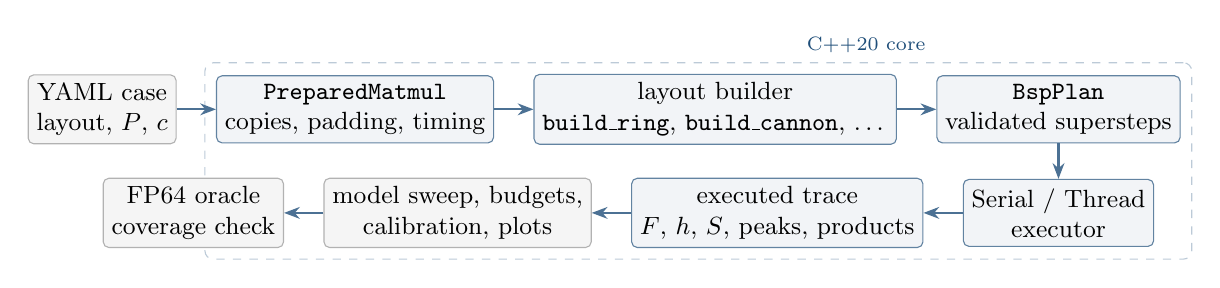
\begin{tikzpicture}[
  font=\small,
  box/.style={draw=accent!70, fill=accent!6, rounded corners=2pt, align=center, minimum height=8.5mm, inner sep=3pt},
  py/.style={box, draw=gray!60, fill=gray!8},
  arr/.style={-{Stealth[length=2mm]}, thick, color=accent!80},
  node distance=4.5mm and 5mm]
  \node[py]  (cfg)  {YAML case\\ layout, $P$, $c$};
  \node[box, right=of cfg] (job)  {\code{PreparedMatmul}\\ copies, padding, timing};
  \node[box, right=of job] (bld)  {layout builder\\ \code{build\_ring}, \code{build\_cannon}, \dots};
  \node[box, right=of bld] (plan) {\code{BspPlan}\\ validated supersteps};
  \node[box, below=of plan] (exe) {Serial / Thread\\ executor};
  \node[box, left=of exe] (tr)  {executed trace\\ $F$, $h$, $S$, peaks, products};
  \node[py, left=of tr] (an)  {model sweep, budgets,\\ calibration, plots};
  \node[py, left=of an] (ora) {FP64 oracle\\ coverage check};
  \draw[arr] (cfg) -- (job);
  \draw[arr] (job) -- (bld);
  \draw[arr] (bld) -- (plan);
  \draw[arr] (plan) -- (exe);
  \draw[arr] (exe) -- (tr);
  \draw[arr] (tr) -- (an);
  \draw[arr] (an) -- (ora);
  \begin{scope}[on background layer]
    \node[draw=accent!30, dashed, rounded corners=3pt, fit=(job)(bld)(plan)(exe)(tr), inner sep=4pt,
          label={[font=\scriptsize\color{accent}]above right:C++20 core}] {};
  \end{scope}
\end{tikzpicture}
\caption{Data flow. Grey boxes are Python, blue boxes C++. A layout only declares a plan; the same
interpreter, executors, memory ledger and trace serve all layouts.}
\label{fig:arch}
\end{figure}

\paragraph{Own work and external components}
The plan runtime, executors, GEMM kernel, layout builders, memory ledger, trace format, coverage validator
and the modelling and measurement pipeline are the team's own code; no BLAS or MPI library is used.
External components are limited to pybind11 and scikit-build-core for the extension, GoogleTest for the
native tests, and NumPy, PyYAML and matplotlib in Python, with NumPy computing the FP64 reference. The
ring, Cannon and 2.5D algorithms follow the cited literature; the 2.5D-direct schedule and the bundling
and merging optimisations of \cref{sec:opt} are our own design for the common row distribution.

\subsection{Layouts}
\label{sec:layouts}

\cref{fig:layouts} sketches the four schedules. For each one we derived closed-form counts before
implementation, and the tests assert them against the executed traces.

\paragraph{1D ring}
Node $r$ keeps its rows of $A$ and $C$ and initially holds row block $r$ of $B$. In round $t$ it computes
$C_r \mathrel{+}= A_r[:,k]\,B_k$ with $k=(r-t)\bmod P$ and passes its $B$ block to node $r+1$. The ring
works directly on the common distribution and needs no conversion; its counts are $S=P$,
$\Ccrit=(P-1)N^2/P$ and $\Ctot=(P-1)N^2$.

\paragraph{2D Cannon}
With $P=q^2$ and tile side $b=N/q$, the rows of $A$ and $B$ are first converted into a $q\times q$ tile
grid. An initial skew sends $A_{ij}$ to $(i,j-i)$ and $B_{ij}$ to $(i-j,j)$; in each of $q$ rounds every
node multiplies its tiles and shifts $A$ left and $B$ up. The native schedule has $S=q+1$ and
$\Ccrit=2qb^2=2\sqrt P\,N^2/P$. Converting rows to tiles and back adds $3(q-1)/q$ units of $N^2/P$ to the
critical path.

\paragraph{2.5D with a base layer}
With $P=cq^2$ and $c\mid q$, the nodes form $c$ layers of $q\times q$ grids. Rows are gathered into tiles
on the base layer and broadcast to the other layers along binary trees. Layer $\ell$ then runs rounds
$[\ell R,(\ell+1)R)$ of Cannon's schedule with $R=q/c$, so each block product $(i,k,j)$ is executed
exactly once across the layers. The partial $C$ tiles are summed back to the base layer along a binary
tree, which adds $(c-1)N^2$ FLOPs, and converted to rows. With $c=1$ the route reduces exactly to Cannon.

\paragraph{2.5D-direct}
The common distribution already spreads the inputs over all $P$ nodes, so there is no need to route them
through the base layer. In 2.5D-direct every row shard sends its pieces of $A$ and $B$ straight to the
matching tiles on all $c$ layers in a single exchange. After the layered Cannon rounds, each layer sends
its partial $C$ tiles straight to the row owners, which sum the $c$ contributions (a reduce-scatter). The
gather, both trees and the output conversion disappear. Counting words per node gives $2c$ units of
$N^2/P$ for replication, $2c$ for the skew, $2c(R-1)$ for the shifts and $c$ for the reduce-scatter, so
\begin{equation}
\Ccrit^{\text{direct}} = \big(3c + 2\sqrt{P/c}\,\big)\,N^2/P .
\label{eq:direct}
\end{equation}

\begin{figure}[t]
\centering
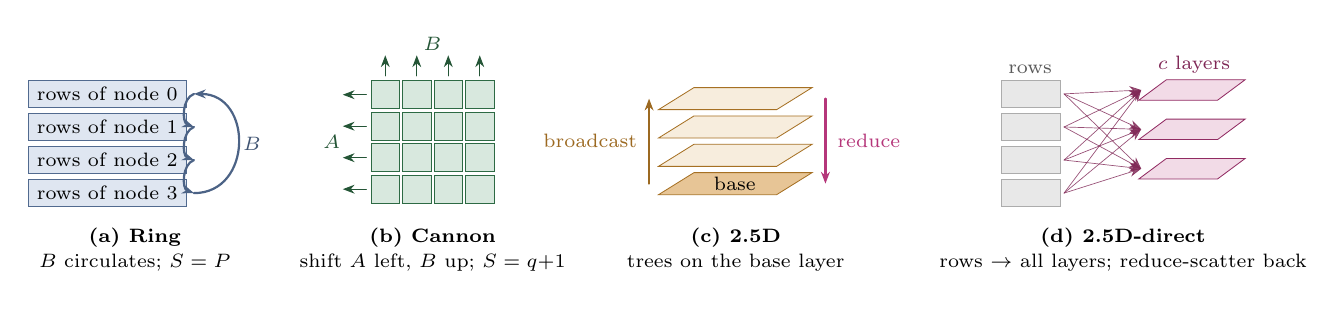
\begin{tikzpicture}[font=\scriptsize, >={Stealth[length=1.5mm]}, line cap=round]
  % ---------------- (a) ring
  \begin{scope}
    \foreach \i in {0,...,3} {
      \fill[ringc!22, draw=ringc!75!black, line width=0.3pt] (0,-\i*0.42) rectangle (2.0,-\i*0.42-0.34);
      \node at (1.0,-\i*0.42-0.17) {rows of node \i};
    }
    \foreach \i in {0,1,2}
      \draw[->, thick, ringc!70!black] (2.1,-\i*0.42-0.17) to[bend right=70] (2.1,-\i*0.42-0.59);
    \draw[->, thick, ringc!70!black] (2.1,-1.43) .. controls (2.85,-1.43) and (2.85,-0.17) .. (2.1,-0.17);
    \node[anchor=west, ringc!60!black] at (2.6,-0.8) {$B$};
  \end{scope}
  \node[align=center] at (1.35,-2.15) {\textbf{(a) Ring}\\[1pt] $B$ circulates; $S=P$};
  % ---------------- (b) cannon
  \begin{scope}[xshift=4.35cm]
    \foreach \i in {0,...,3} \foreach \j in {0,...,3}
      \fill[cannonc!20, draw=cannonc!75!black, line width=0.3pt] (\j*0.4,-\i*0.4) rectangle ++(0.36,-0.36);
    \foreach \i in {0,...,3} \draw[->, cannonc!60!black] (-0.06,-\i*0.4-0.18) -- (-0.36,-\i*0.4-0.18);
    \foreach \j in {0,...,3} \draw[->, cannonc!60!black] (\j*0.4+0.18,0.06) -- (\j*0.4+0.18,0.32);
    \node[cannonc!60!black] at (-0.5,-0.78) {$A$};
    \node[cannonc!60!black] at (0.78,0.47) {$B$};
  \end{scope}
  \node[align=center] at (5.13,-2.15) {\textbf{(b) Cannon}\\[1pt] shift $A$ left, $B$ up; $S=q{+}1$};
  % ---------------- (c) 2.5D
  \begin{scope}[xshift=8.0cm, yshift=-1.45cm]
    \foreach \l in {3,2,1,0} {
      \pgfmathsetmacro{\shade}{\l==0 ? 50 : 16}
      \fill[tdc!\shade, draw=tdc!80!black, line width=0.3pt]
        (0,\l*0.36) -- ++(1.5,0) -- ++(0.45,0.28) -- ++(-1.5,0) -- cycle;
    }
    \node at (0.97,0.14) {base};
    \draw[->, thick, tdc!75!black] (-0.12,0.14) -- (-0.12,1.22);
    \node[anchor=east, tdc!75!black] at (-0.15,0.68) {broadcast};
    \draw[->, thick, directc] (2.12,1.22) -- (2.12,0.14);
    \node[anchor=west, directc] at (2.15,0.68) {reduce};
  \end{scope}
  \node[align=center] at (8.98,-2.15) {\textbf{(c) 2.5D}\\[1pt] trees on the base layer};
  % ---------------- (d) direct
  \begin{scope}[xshift=12.35cm]
    \foreach \i in {0,...,3}
      \fill[gray!18, draw=gray!65, line width=0.3pt] (0,-\i*0.42) rectangle (0.75,-\i*0.42-0.34);
    \node[gray!70!black] at (0.37,0.14) {rows};
    \foreach \l/\y in {2/-0.25,1/-0.75,0/-1.25}
      \fill[directc!18, draw=directc!80!black, line width=0.3pt]
        (1.75,\y) -- ++(1.0,0) -- ++(0.35,0.26) -- ++(-1.0,0) -- cycle;
    \node[directc!70!black] at (2.45,0.2) {$c$ layers};
    \foreach \yr in {-0.17,-0.59,-1.01,-1.43}
      \foreach \yl in {-0.12,-0.62,-1.12}
        \draw[->, directc!70!black, line width=0.25pt, opacity=0.8] (0.8,\yr) -- (1.78,\yl);
  \end{scope}
  \node[align=center] at (13.9,-2.15) {\textbf{(d) 2.5D-direct}\\[1pt] rows $\to$ all layers; reduce-scatter back};
\end{tikzpicture}
\caption{The four schedules. All start and end in the common row distribution; (b), (c) and (d) convert
to and from tiles inside the measured route.}
\label{fig:layouts}
\end{figure}

\subsection{Optimisations}
\label{sec:opt}

\begin{itemize}
\item \textbf{Shared blocked kernel.} All layouts call one rectangular FP32 GEMM with a fixed $32\times32$
      tile, row strides and tail handling, so that differences between layouts come from data movement
      rather than from different kernels.
\item \textbf{Allocation-free execution.} Buffers and message slots are allocated when the plan is
      finalised. A global allocation hook in the tests confirms that neither the caller nor any worker
      allocates during the first or any later execution, and that a failed batch can be retried.
\item \textbf{Bundled conversion and delivery merging.} The conversions of $A$ and $B$ share one exchange,
      so each node pair exchanges a single message per step, and a superstep that only receives or copies
      is merged into the next one. At $P=256$ this lowers Cannon's supersteps from 23 to 20 and its
      messages from 19\,680 to 15\,840, and the supersteps of base-layer 2.5D from 15 to 11, without
      changing any FLOP or word count.
\item \textbf{Direct replication.} 2.5D-direct (\cref{sec:layouts}) is our main algorithmic optimisation;
      \cref{sec:direct} quantifies its effect.
\end{itemize}

% ================================================================ 4
\section{Correctness Verification}
\label{sec:verify}

Because the analysis rests on executed counts, correctness is checked at three levels: the numerical
result, the schedule and the communication protocol.

\paragraph{Numerical results}
Inputs are generated from a fixed seed (5206) and stored as FP32; an independent NumPy product in FP64
serves as the reference. Every element must satisfy $|x-x_{\mathrm{ref}}|\le10^{-4}+10^{-3}|x_{\mathrm{ref}}|$.
Unit tests add zero, identity, all-ones and sign-cancelling matrices, $P=1$, and the non-divisible sizes
$n=17,65,257$ that exercise padding and cropping.

\paragraph{Schedules}
Each GEMM records its block triple $(i,k,j)$, and an independent validator confirms that every product of
the block grid is executed exactly once, so that no layout can appear cheap by skipping or duplicating
work. The tests compare the executed counts with the closed forms of \cref{sec:layouts}, check message
routes, and confirm that 2.5D with $c=1$ reproduces Cannon's output and schedule.

\paragraph{Protocol}
The plan rejects unmatched, duplicated or unconsumed messages, out-of-bounds views and invalid grids (for
example $P=64$, $c=3$) before execution, and an experiment profile containing an invalid case fails before
any output is written.

\paragraph{Test suite and formal runs}
The submitted commit contains 74 GoogleTest definitions and 178 pytest functions, many parametrised over
worker counts and grids. Continuous integration builds the extension, runs both suites and a smoke
experiment on every push; for the submitted commit all 123 native test cases pass, and 513 of the 514
collected Python cases pass with one skipped. All 24 main, 6 ablation and
9 padding configurations pass the FP64 check with a largest Frobenius relative error of
$4.3\times10^{-7}$, as does every timed sample on both hosts. Additional runs of both 2.5D routes at
$P=256$ ($c=4$), $P=108$ ($c=3$), $P=125$ ($c=5$) and $P=216$ ($c=6$), including replication factors
that are not powers of two, pass the same rule and the coverage validator. The executed counts of the
submitted commit are identical, field by field, when regenerated on a second host.

% ================================================================ 5
\section{Experimental Method}
\label{sec:setup}

The design in \cref{tab:grid} was fixed in the proposal, apart from the 2.5D-direct ablation, which was
added later on the same grid. It yields two kinds of evidence.
\emph{Modelled cost:} each of the 24 main configurations is executed once on real data and its trace
saved. The 192 cost scenarios are priced from these traces without new arithmetic, and the two budgets
filter the same results into $3\times3\times4\times2\times2=144$ selection cells, each a combination of $n$,
$P$, $\gamma$, $\lambda$ and $\mu$; the ablation profile adds 2.5D-direct at $P=64$ and $256$.
\emph{Measured time:} formal timing requires one physical core per logical node, $P\le H\le$ physical
cores, which rules out the grids of the model sweep; as planned in the proposal, Ring and Cannon are timed
at $P=H=1$ and $P=H=4$.

\begin{table}[htb]
\centering
\caption{Experimental design. All entries except the 2.5D-direct ablation were fixed in the proposal.}
\label{tab:grid}
\small
\begin{tabular}{@{}ll@{}}
\toprule
Dimension & Values \\
\midrule
Matrix size $n$ & 256, 512, 1024 (padding check: 17, 65, 257) \\
Logical nodes $P$ & 16, 64, 256 \\
Layouts & $P=16$: Ring, Cannon \\
 & $P=64,256$: Ring, Cannon, 2.5D ($c=4$), 2.5D-direct ($c=4$, ablation) \\
Communication cost $\gamma$ & 1, 10, 100, 1000 FLOPs per word \\
Synchronisation cost $\lambda$ & $10^2$, $10^4$ FLOPs per superstep \\
Memory budget & $M_{\mathrm{cap}}=\mu N^2/P$ words, $\mu\in\{8,32\}$ \\
Timing subset & Ring and Cannon, $P=H=1$ and $P=H=4$, 5 warm-ups, 15 repetitions \\
\bottomrule
\end{tabular}
\end{table}

\paragraph{Timing protocol}
The timed interval runs from common rows to common rows after preallocation and includes conversion,
message copies, GEMMs and barriers; input generation, allocation, validation and file I/O are excluded. We
report the median of 15 repetitions after 5 warm-ups~\cite{hoefler2015}; the interquartile range is below
7\% of the median for every ARM64 run and every run at $n=1024$, and at most 23\% (four-worker Cannon on
x86 at $n=256$). Before any
matrix run, independent micro-benchmarks fix $w$ (GEMM), $g$ (copy) and $l$ (empty superstep); the model is
then evaluated on the full runs without per-case refitting, so its residuals are held-out errors.

\paragraph{Hosts}
The main measurements run the submitted commit on an Intel Core i5-13600K (6 performance and 8 efficiency
cores, 20 hardware threads, 24\,MB L3) under WSL2 Ubuntu 24.04, compiled with GCC 16.2 in a Release
build. Worker threads are persistent
but not pinned, so the scheduler may place them on either core type; the one-minute load average was
0.12--0.19 before and after each timed run. For a cross-platform comparison, Ring and Cannon were also
timed on an 8-core Apple-silicon machine (macOS, Apple LLVM 21) at revision \code{9fc781b}. That revision
predates bundling and delivery merging, so its Cannon route at $P=4$ has 9 supersteps instead of 6 but
identical FLOP and word counts.

% ================================================================ 6
\section{Results}
\label{sec:results}

\subsection{Communication and synchronisation}

\cref{tab:counts} lists the executed counts at $n=1024$, normalised by $n^2/P$ so that they are comparable
across $P$. All layouts perform the same $2N^3$ GEMM FLOPs; the 2.5D routes add $(c-1)N^2$ reduction
additions, 0.15\% of the work, so the layouts differ almost entirely in communication, synchronisation and
memory.

\begin{table}[t]
\centering
\caption{Executed counts at $n=1024$ (submitted commit). \emph{Native} excludes the conversion from and to
the common distribution; \emph{common} is the full row-to-row route. Peak is the largest live per-node
payload.}
\label{tab:counts}
\small
\begin{tabular}{@{}rl rr rr rr r@{}}
\toprule
& & \multicolumn{2}{c}{$\Ccrit/(n^2/P)$} & \multicolumn{2}{c}{Supersteps $S$} & \multicolumn{2}{c}{Common route} & \\
\cmidrule(lr){3-4}\cmidrule(lr){5-6}\cmidrule(lr){7-8}
$P$ & Layout & native & common & native & common & $\Ctot/n^2$ & messages & Peak$/(n^2/P)$ \\
\midrule
16  & Ring        & 15.00 & 15.00 & 16 & 16 & 15.00 & 240 & 5.00 \\
    & Cannon      & 8.00  & 10.25 & 5  & 8  & 9.75  & 216 & 7.25 \\
\rowcolor{rowgray}
64  & Ring        & 63.00 & 63.00 & 64 & 64 & 63.00 & 4\,032 & 5.00 \\
\rowcolor{rowgray}
    & Cannon      & 16.00 & 18.63 & 9  & 12 & 18.38 & 1\,904 & 7.13 \\
\rowcolor{rowgray}
    & 2.5D        & 44.00 & 56.00 & 7  & 10 & 17.95 & 696 & 28.00 \\
\rowcolor{rowgray}
    & 2.5D-direct & 20.00 & 20.00 & 5  & 5  & 17.81 & 2\,112 & 28.00 \\
256 & Ring        & 255.00 & 255.00 & 256 & 256 & 255.00 & 65\,280 & 5.00 \\
    & Cannon      & 32.00 & 34.81 & 17 & 20 & 34.69 & 15\,840 & 7.06 \\
    & 2.5D        & 52.00 & 64.00 & 8  & 11 & 26.99 & 5\,424 & 28.00 \\
    & 2.5D-direct & 28.00 & 28.00 & 6  & 6  & 26.95 & 17\,280 & 28.00 \\
\bottomrule
\end{tabular}
\end{table}

The ring's communication and supersteps both grow linearly with $P$: at $P=256$ it moves $255\,n^2$ words
in total, seven times more than Cannon, and needs 256 barriers. Cannon follows its $2\sqrt P$ law exactly
in the native schedule, and the conversion from and to rows adds less than three units at every $P$.

Replication lowers the \emph{total} traffic as intended: at $P=256$ base-layer 2.5D moves 22\% fewer words
than Cannon, and its multiply phase needs only 8 critical units against Cannon's 30. Its critical
communication, however, is 84\% \emph{higher}. \cref{fig:phases} shows why. The gather onto the base layer,
the tree broadcast, the tree reduction and the output conversion together cost 48 of its 64 units, and
they funnel all data through the base layer. Base nodes are the busiest nodes in steps worth 36 of these
units: they receive the gathered rows, send to two layers at once at the root of the broadcast tree,
receive from two layers at the root of the reduction tree and scatter the result back to rows. The
remaining 12 units come from inner tree steps in which half of the nodes are idle. Traffic that is cheap in total therefore
appears in full on the critical path.

\begin{figure}[t]
\centering
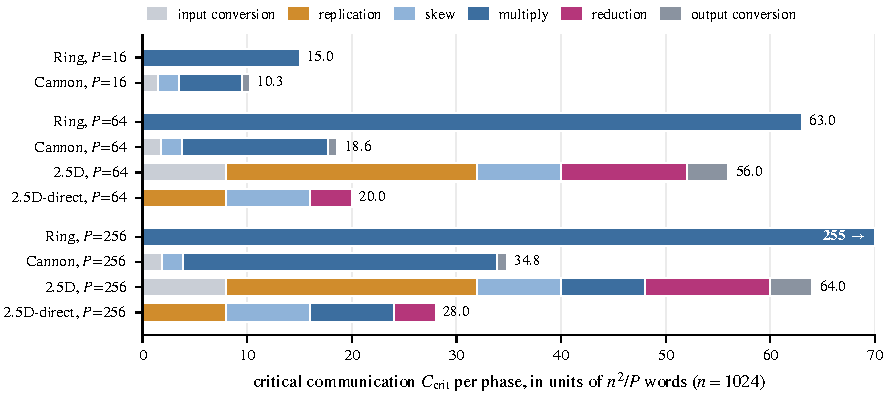
\includegraphics[width=\textwidth]{figures/phase_breakdown.pdf}
\caption{Critical communication per phase at $n=1024$. Base-layer 2.5D spends 48 of its 64 units in the
gather, tree broadcast, tree reduction and output conversion around the base layer; 2.5D-direct replaces
them with one all-node exchange in each direction.}
\label{fig:phases}
\end{figure}

\subsection{Removing the base-layer bottleneck}
\label{sec:direct}

2.5D-direct spreads the same replication over all $P$ nodes. At $P=256$ it needs 8 critical units for
replication, 8 for the skew, 8 for the multiply phase and 4 for the reduce-scatter, exactly as
\cref{eq:direct} predicts. Its critical communication falls from 64 to 28 units, 20\% below Cannon, and its
supersteps from 11 to 6, against Cannon's 20. The total traffic barely changes (26.95 against 26.99 $n^2$
words), because the same data must still move; what improves is its distribution over the nodes. The price is more and smaller messages
(17\,280 against 5\,424), which the BSP model does not charge. At $P=64$, where each layer performs a single
Cannon round, 2.5D-direct sends slightly more critical words than Cannon (20 against 18.6 units) and
its advantage is the shorter schedule of 5 supersteps instead of 12.

\subsection{Memory budgets and layout selection}

\begin{figure}[t]
\centering
\begin{subfigure}[b]{0.47\textwidth}
  \centering
  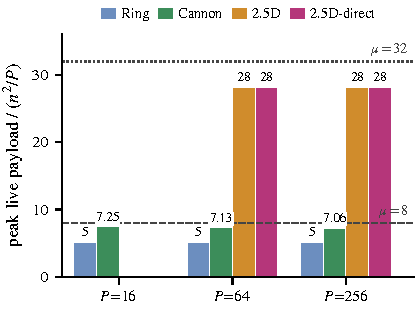
\includegraphics[width=\textwidth]{figures/peak_memory.pdf}
  \caption{Peak live payload per node at $n=1024$.}
  \label{fig:memory}
\end{subfigure}\hfill
\begin{subfigure}[b]{0.5\textwidth}
  \centering
  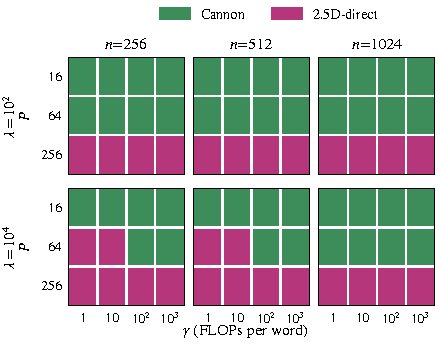
\includegraphics[width=\textwidth]{figures/layout_selection.pdf}
  \caption{Cheapest feasible layout, budget $\mu=32$.}
  \label{fig:selection}
\end{subfigure}
\caption{Memory feasibility and end-to-end layout selection. With $\mu=8$ both 2.5D routes are infeasible
and Cannon wins every cell, so only $\mu=32$ is shown.}
\label{fig:memsel}
\end{figure}

The normalised peaks in \cref{fig:memory} are independent of the matrix size and almost independent of $P$.
The ring needs 5 units for its row shards, the circulating $B$ block and its message buffers, and Cannon
about 7 because row shards, tiles and conversion buffers are live at the same time. Both 2.5D routes need
28 units, since every node also holds replicated $A$ and $B$ tiles, a partial $C$ tile and the messages
that move them. They therefore exceed the tight budget and fit only the loose one.

Under $\mu=8$ memory rules out both 2.5D routes, and Cannon is cheaper than the ring in all 72 cells. With the three layouts of the proposal, Cannon wins 141 of all 144 cells; base-layer 2.5D wins
only three, all under $\mu=32$ at $P=256$ and $\lambda=10^4$ with small $n$ and $\gamma$, where nine saved
barriers outweigh its extra words. Adding 2.5D-direct moves 28 cells to it (\cref{fig:selection}): every
loose-budget cell at $P=256$, with model costs between 0.2\% and 41\% below Cannon and the margin growing
as $n$ shrinks and $\lambda$ grows, and the four cells at $P=64$ with $\lambda=10^4$, $\gamma\le10$ and
$n\le512$. The ring never wins: its footprint is the smallest, but its $\Theta(P)$ words and supersteps
dominate at every $\gamma$ and $\lambda$ we tested.

\subsection{Measured performance}
\label{sec:measure}

\begin{table}[t]
\centering
\caption{End-to-end medians in ms on both hosts. Speedup compares $P=H=4$ with the same layout at $P=H=1$;
the residual (measured $-$ predicted)/measured refers to $P=H=4$. Positive residuals mean that the
calibrated model is too optimistic.}
\label{tab:timing}
\small
\begin{tabular}{@{}rl rrrr rrrr@{}}
\toprule
& & \multicolumn{4}{c}{x86, \code{0b8b2b8}} & \multicolumn{4}{c}{ARM64, \code{9fc781b}} \\
\cmidrule(lr){3-6}\cmidrule(l){7-10}
$n$ & Layout & $P=1$ & $P=4$ & Speedup & Residual & $P=1$ & $P=4$ & Speedup & Residual \\
\midrule
256  & Ring   & 1.463   & 1.419  & $1.03\times$ & $+13.3\%$ & 2.330   & 1.053  & $2.21\times$ & $+24.6\%$ \\
     & Cannon & 1.505   & 1.852  & $0.81\times$ & $+10.7\%$ & 2.333   & 1.155  & $2.02\times$ & $+14.5\%$ \\
\rowcolor{rowgray}
512  & Ring   & 13.483  & 5.158  & $2.61\times$ & $+23.6\%$ & 18.785  & 5.465  & $3.44\times$ & $+3.5\%$ \\
\rowcolor{rowgray}
     & Cannon & 13.471  & 4.998  & $2.70\times$ & $+12.5\%$ & 18.751  & 5.692  & $3.29\times$ & $+3.5\%$ \\
1024 & Ring   & 111.787 & 31.800 & $3.52\times$ & $+19.6\%$ & 165.181 & 44.439 & $3.72\times$ & $+7.7\%$ \\
     & Cannon & 112.499 & 32.298 & $3.48\times$ & $+19.4\%$ & 165.302 & 41.071 & $4.02\times$ & $-0.6\%$ \\
\bottomrule
\end{tabular}
\end{table}

\begin{figure}[t]
\centering
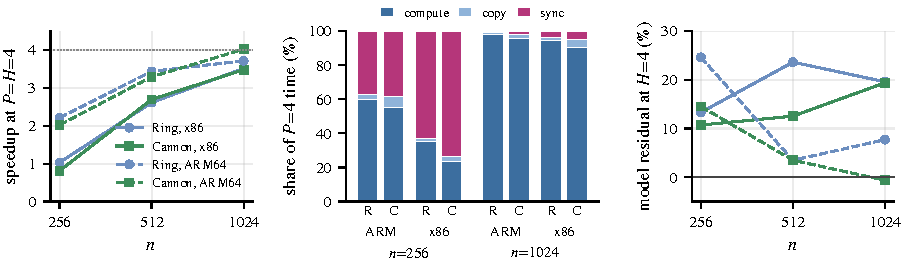
\includegraphics[width=\textwidth]{figures/measurement.pdf}
\caption{Prepared measurements at $P=H=4$. Left: speedup over the same layout at $P=H=1$ (solid: x86,
dashed: ARM64). Centre: share of the measured compute, copy and synchronisation components (R: Ring,
C: Cannon). Right: signed residual of the calibrated BSP model on held-out runs.}
\label{fig:measure}
\end{figure}

\cref{tab:timing} and \cref{fig:measure} summarise the timed subset. With one worker both layouts perform
the same computation and agree within 3\%, at 19--23\,GFLOP/s on x86 and 13--14\,GFLOP/s on ARM64.

\paragraph{Scaling}
At $n=1024$ four workers reach a $3.5\times$ speedup on x86, with 87--88\% parallel efficiency and up to
67.5\,GFLOP/s, and $3.7$--$4.0\times$ on ARM64. The slightly superlinear value for Cannon on ARM64 is
consistent with the higher GEMM throughput on smaller blocks discussed under model fidelity below. At
$n=256$ the speedup falls to $2.0$--$2.2\times$ on ARM64 and vanishes on x86, where Cannon with four
workers takes 23\% longer than with one and the ring merely breaks even.

\paragraph{Synchronisation dominates small problems}
The phase breakdown explains this behaviour. At $n=256$ synchronisation takes 63--74\% of the four-worker
time on x86 and 37--38\% on ARM64, but less than 5\% at $n=1024$ on both hosts. The calibrated parameters
quantify the imbalance: on x86, $w=4.6\times10^{-11}$\,s per FLOP, $g=7.2\times10^{-11}$\,s per word and
$l=2.1\times10^{-4}$\,s per superstep, i.e.\ $\gamma\approx1.6$ and $\lambda\approx4.6\times10^6$; on ARM64,
$\gamma\approx2.7$ and $\lambda\approx4.9\times10^5$. Moving a word through shared memory therefore costs
about as much as a FLOP, whereas a superstep costs $5\times10^5$ to $5\times10^6$ FLOPs. Consequently the
ring, with four supersteps instead of Cannon's six, needs 23\% less time than Cannon at $n=256$ on x86.

\paragraph{No robust ranking at large $n$}
For $n\ge512$ the measured times of the two layouts differ by at most 7.6\%, and the sign of the
difference changes between hosts: on ARM64 Cannon needs 7.6\% less time than the ring at $n=1024$, with a
shorter compute component (39.4 against 43.6\,ms), whereas on x86 the ring needs 1.5\% less time at the
same size. The model places the two layouts within 2\% of each other at $n=1024$, because Cannon's grid at
$P=4$ is only $2\times2$. The measured differences most likely stem from how each host's memory hierarchy
handles the different GEMM shapes ($512\times512\times512$ blocks for Cannon, $256\times256$ by
$256\times1024$ for the ring) rather than from the communication of the layouts.

\paragraph{Model fidelity}
On ARM64 the calibrated model predicts the four-worker time within 4\% at $n=512$ and for Cannon at
$n=1024$. On x86 it is consistently optimistic, by 11--24\% with four workers and by 10--14\% even with one
worker at $n\ge512$. The single-worker rates show why: GEMM throughput falls from 22.3 to 19.1\,GFLOP/s on
x86, and from 14.4 to 13.0\,GFLOP/s on ARM64, as $n$ grows from 256 to 1024, whereas $w$ is calibrated once
on small, cache-resident micro-benchmarks. A constant per-FLOP cost cannot represent this memory-hierarchy
effect, so we use the model to rank layouts rather than to predict absolute times.

% ================================================================ 7
\section{Analysis and Discussion}
\label{sec:discussion}

\paragraph{When replication pays}
\cref{eq:direct} makes the trade-off explicit. The term $3c$ is a fixed price for replication, skew and
reduction that does not shrink with $P$, while the term $2\sqrt{P/c}$ grows more slowly than Cannon's
$2\sqrt P$ by a factor $\sqrt c$. For $c=4$ the comparison is $12+\sqrt P$ against $2\sqrt P$ plus
Cannon's conversion of $3(1-1/\sqrt P)$, and the two cross at $\sqrt P\approx9.3$, between our grids
$P=64$ and $P=256$; this is exactly where the measured counts change order. Fewer supersteps move the
crossover to smaller $P$ when barriers are expensive, because 2.5D-direct needs $\sqrt{P}/c^{3/2}+4$
supersteps against Cannon's $\sqrt P+4$; this is why it already wins the $\lambda=10^4$, small-$\gamma$
corner at $P=64$. Large $n$ moves the balance back towards Cannon, because the extra reduction FLOPs and
the extra words of 2.5D-direct at $P=64$ both grow with $n^2$, while the saving in barriers is fixed; at
$n=1024$ Cannon regains that corner, by as little as 0.005\% at $\gamma=1$.

\paragraph{The schedule matters as much as the algorithm}
Our first 2.5D implementation followed the common textbook description, in which a base layer gathers,
broadcasts and reduces. Measured by total traffic, the usual communication-avoiding metric, it succeeded;
measured by the critical path, it failed, because its collectives funnel all data through the base layer,
a quarter of the nodes. The per-phase breakdown of the formal run exposed this, and replacing the trees by
direct exchanges more than halved the critical communication. More generally, an asymptotic saving in
words is realised only if the schedule keeps the communication balanced across nodes.

\paragraph{Memory is the binding constraint}
In every run the peak payload of both 2.5D routes is exactly $7c$ units of $N^2/P$: 28 for $c=4$ in the
sweep, and 21, 35 and 42 for $c=3,5,6$ in the additional checks. A budget $\mu$ therefore admits a
replication factor of at most $\lfloor\mu/7\rfloor$, which excludes replication entirely at $\mu=8$ and
allows $c=4$ at $\mu=32$. This is the trade-off expressed by the lower bound
$\Omega\big(n^3/(P\sqrt M)\big)$ on per-node communication~\cite{ballard2011,ballard2014}: Cannon already
attains it for $M=\Theta(n^2/P)$, and fewer words are possible only with more memory.

\paragraph{From the model to real machines}
Our sweep spans $\lambda\le10^4$, but the hosts exhibit $\lambda$ between $4.9\times10^5$ and
$4.6\times10^6$. The reason is the executor: each superstep consists of three blocking dispatches to a
thread pool whose workers sleep on a condition variable, so every barrier pays an operating-system wake-up
rather than a memory fence; the x86 host, running under WSL2, pays 5.7 times more per superstep than the
ARM64 host. In this latency-dominated regime
the number of supersteps decides, which favours both replicated layouts and 2.5D-direct in particular. On
a distributed-memory cluster the balance would shift towards larger $\gamma$, and a per-message cost would
appear that the BSP model omits; since 2.5D-direct sends three times as many messages as base-layer 2.5D,
a LogP-style model~\cite{culler1993} would be needed to settle that comparison.

% ================================================================ 8
\section{Limitations}
\label{sec:limits}

Wall-clock timing requires one physical core per logical node, whereas the 2.5D routes need $P\ge64$;
their evidence therefore rests on correctness checks, executed counts and the BSP model. The model idealises the network, charging words and barriers but not per-message
overhead or contention, and the sweep is limited to square FP32 matrices with a single replication factor,
$c=4$.

% ================================================================ 9
\section{Conclusion}
\label{sec:conclusion}

Executing all layouts on one BSP runtime and pricing their exact traces gives a clear answer to our
question. Cannon is the robust default: it fits the tight memory budget, its critical communication per
node falls as $2n^2/\sqrt P$ words, and it is the cheapest layout in all 72 tight-budget cells and in 116
of the 144 cells overall. The ring has the smallest footprint but loses everywhere, because its words and
supersteps grow linearly with $P$. Replication pays reliably only when three conditions hold together: memory for
$7c$ units per node, a grid large enough for the $\sqrt c$ saving to exceed the fixed replication cost, and
a schedule that spreads replication and reduction over all nodes. Our 2.5D-direct schedule satisfies the
last condition and lowers critical communication by 20\% and supersteps by 70\% relative to Cannon at
$P=256$, whereas the textbook base-layer route almost never wins. The measurements confirm good scaling at
$n=1024$ on both hosts, but they also show that on shared-memory hosts barriers rather than data movement
are the dominant overhead, which is precisely the regime in which fewer supersteps matter most.

% ================================================================ appendix-like sections
\section*{Reproduction}
\addcontentsline{toc}{section}{Reproduction}

The repository README gives full instructions. With a C++20 compiler, CMake~$\ge$3.21 and \code{uv}
(Python 3.12), the following commands build, test and reproduce the main results from a clean checkout of
\code{0b8b2b8}.

\begin{small}
\begin{verbatim}
git clone --recurse-submodules https://github.com/ceg5206-g7/dmm && cd dmm
git checkout 0b8b2b8
uv sync --locked && uv run --locked pytest -q                  # build + Python tests
uv run cmake --preset release && uv run cmake --build --preset release --parallel
uv run ctest --preset release --no-tests=error                  # C++ tests
uv run dmm generate --config configs/dataset.yaml              # seed 5206
uv run dmm generate --config configs/dataset_padding.yaml      # n = 17, 65, 257
uv run dmm model    --config configs/model.yaml                # 24 traces, 192 scenarios
uv run dmm model    --config configs/model_direct.yaml         # + 2.5D-direct ablation
uv run dmm model    --config configs/model_padding.yaml        # 9 padding configurations
uv run dmm measure  --config configs/measure_serial.yaml
uv run dmm measure  --config configs/measure_threaded.yaml --baseline results/measure_serial
\end{verbatim}
\end{small}

\noindent The figures in this report are drawn by \code{report/make\_figures.py} from unmodified copies
of the result CSV files, stored in \code{report/data}.

\section*{Member Contributions}
\addcontentsline{toc}{section}{Member Contributions}

\begin{center}
\small
\begin{tabularx}{\textwidth}{@{}l X@{}}
\toprule
Member & Contribution \\
\midrule
Yang Tingjie   & Proposed the project idea. \\
Yang Hanwei    & Implemented the 1D ring and 2.5D layouts and the 2.5D-direct ablation, the bundled conversion,
                 delivery merging and live-payload peak accounting; published the \code{0b8b2b8} result release and
                 the x86 low-load result set; produced the video. \\
Meng Xiangrun  & Debugging and review of results; prepared this report and its figures and checked the reported
                 numbers against the released result files. \\
Jin Ceyang     & Built the project framework: BSP plan runtime and executors, shared GEMM kernel, collectives,
                 memory ledger, traces and coverage validator, measurement and calibration pipeline, and the
                 documentation site; implemented Cannon's algorithm; published the ARM64 result release
                 (\code{9fc781b}). \\
\bottomrule
\end{tabularx}
\end{center}

\section*{Use of AI Tools}
\addcontentsline{toc}{section}{Use of AI Tools}

Claude (Anthropic) was used to draft and edit the text of this report, to write the script that redraws
the figures from the published CSV files, and to prepare the slides, script and figures of the video; the
video narration was synthesised with Kokoro TTS. AI coding assistants were also used for parts of the
source code and the experiment scripts. The team reviewed all AI-generated code and text: the code is
validated by the test suite and the FP64 and coverage checks of \cref{sec:verify}, and every number in
this report was taken from the released result files and checked against them.

% ================================================================ references
\begin{thebibliography}{9}
\setlength{\itemsep}{1pt}
\small
\bibitem{valiant1990} L.~G. Valiant. A bridging model for parallel computation. \emph{Communications of the ACM}, 33(8):103--111, 1990.
\bibitem{hill1998} J.~M.~D. Hill, B.~McColl, D.~C. Stefanescu, M.~W. Goudreau, K.~Lang, S.~B. Rao, T.~Suel, T.~Tsantilas and R.~H. Bisseling. BSPlib: The BSP programming library. \emph{Parallel Computing}, 24(14):1947--1980, 1998.
\bibitem{culler1993} D.~Culler, R.~Karp, D.~Patterson, A.~Sahay, K.~E. Schauser, E.~Santos, R.~Subramonian and T.~von~Eicken. LogP: Towards a realistic model of parallel computation. In \emph{PPoPP}, pages 1--12, 1993.
\bibitem{cannon1969} L.~E. Cannon. \emph{A Cellular Computer to Implement the Kalman Filter Algorithm}. PhD thesis, Montana State University, 1969.
\bibitem{solomonik2011} E.~Solomonik and J.~Demmel. Communication-optimal parallel 2.5D matrix multiplication and LU factorization algorithms. Technical Report UCB/EECS-2011-72, UC Berkeley, 2011.
\bibitem{vandegeijn1997} R.~A. van~de~Geijn and J.~Watts. SUMMA: Scalable universal matrix multiplication algorithm. \emph{Concurrency: Practice and Experience}, 9(4):255--274, 1997.
\bibitem{ballard2011} G.~Ballard, J.~Demmel, O.~Holtz and O.~Schwartz. Minimizing communication in numerical linear algebra. \emph{SIAM J.\ Matrix Anal.\ Appl.}, 32(3):866--901, 2011.
\bibitem{ballard2014} G.~Ballard, E.~Carson, J.~Demmel, M.~Hoemmen, N.~Knight and O.~Schwartz. Communication lower bounds and optimal algorithms for numerical linear algebra. \emph{Acta Numerica}, 23:1--155, 2014.
\bibitem{hoefler2015} T.~Hoefler and R.~Belli. Scientific benchmarking of parallel computing systems. In \emph{SC15}, pages 73:1--73:12, 2015.
\end{thebibliography}

\end{document}
